\documentclass[12pt]{article}
\usepackage{graphicx}

\oddsidemargin  -0.5 cm
\evensidemargin 0.0 cm
\textwidth      6.5in
\headheight     0.0in
\topmargin      -1 cm
\textheight=9in

\newcommand{\s}[1]{{\mbox{\scriptsize #1}}}

\begin{document}

\section{Quick introduction}

This is a study of the effect of systematic alignment uncertainties on
the shape of the $Z' \to \mu\mu$ peak.  It is meant to be a first
approximation of the $Z'$ width uncertainty that feeds into
limit-setting, though I'll point out some ways in which the study
should be improved before it becomes a line in the systematics table
of a $Z'$ paper.

\section{Current situation in muon alignment}

We now have two independent measurements of the DT chamber positions:
one from tracker-tracks propagated to the muon segments (``track-based
alignment'') and the other from in-situ physical measurements of the
chamber positions, together with detailed studies of the internal
chamber geometry from measurements at the construction sites to
connect chamber positions to internal layer positions (``hardware
alignment'').  These two systems agree broadly about the cm-scale
corrections that must be applied to the design geometry, mostly to
account for gravitational sag (Fig.~\ref{fig:tb-hw_wheel0}).  However,
mm-scale differences remain, and these differences have two systematic
trends shown in Fig.~\ref{fig:twist3}: (1) groups of chambers in the
same sector ($\phi$-bin) appear to be coherently rotated such that
wheel~$+$2 chambers are displaced in one direction in $r\phi$ and
wheel~$-$2 chambers are displaced in the other direction in $r\phi$;
(2) the two measurements differ in $z$-scale.  Of these two effects,
only the first (``twist'') is relevant for momentum measurement and
hence $Z'$ resolution.  The twist effect is shown more quantitatively
in Fig.~\ref{fig:twist1}.

\begin{figure}
\includegraphics[width=\linewidth]{tb-hw_wheel0.png}
\caption{Exaggerated graphical view of differences between
  track-based (TB), hardware (HW), and unaligned (IDEAL) chamber
  positions and angles for wheel~0. \label{fig:tb-hw_wheel0}}
\end{figure}

\begin{figure}
\includegraphics[width=\linewidth]{twist3.png}
\caption{Exaggerated graphical view of differences between track-based
  and hardware geometries in the $z$-$\phi$ projection (unrolled muon
  barrel).  Station~4 $z$ positions cannot be measured by tracks (no
  $z$-measuring superlayer). \label{fig:twist3}}
\end{figure}

\begin{figure}
\includegraphics[width=\linewidth]{twist1.png}
\caption{Histogram of differences in chamber positions between
  track-based and hardware methods, separated by wheel.  The ``($x \pm
  y$)~mm'' numbers refer to the mean and RMS of each
  distribution. \label{fig:twist1}}
\end{figure}

The same discrepancy has been studied at the level of raw residuals by
plotting track residuals with the hardware geometry.  This is
equivalent to the chamber position comparison from the two alignments
(Figs.~\ref{fig:tb-hw_wheel0}--\ref{fig:twist1}), except that the
binning is smaller than a chamber, the detector signals have are
minimally processed (no multi-dimensional fits to all alignment
degrees of freedom), and error bars are shown.  A survey of $r\phi$
residuals versus $z$ for station~1 is presented in
Fig.~\ref{fig:twist2}, illustrating the consistent ``twist''-like
slope of all 12 sectors.

\begin{figure}
\includegraphics[width=\linewidth]{twist2.png}
\caption{Global $r\phi$ residuals (also known as local~$x'$) versus
  global $z$ position of the hit.  The blue background is a 2-D
  distribution of the individual hits, the black points with error
  bars is the mean of each vertical slice, and the dashed lines
  indicate chamber boundaries (which are also wheel
  boundaries).  \label{fig:twist2}}
\end{figure}

To demonstrate the consistency of the effect for all sectors and all
stations, the 12 plots in Fig.~\ref{fig:twist2} and the 38 additional
plots from stations~2--4 were fitted with a straight line: one example
fit and the distribution of normalized $\chi^2$ values are in
Fig.~\ref{fig:growth_with_station}.  The slope of each fit
characterizes the twist effect in that sector and station: histograms
of all slopes are presented in Fig.~\ref{fig:growth_with_station2},
where we can see that they are clustered around $-5\times
10^{-3}$~mm/cm, independent of station number.

\begin{figure}
\begin{center}
\includegraphics[height=5 cm]{growth_with_station2.png} \hspace{0.5 cm}
\includegraphics[height=5 cm]{growth_with_station_chi2.png}
\end{center}
\caption{Left: example fit of one of the plots from
  Fig.~\ref{fig:twist2}.  Right: distribution of $\chi^2/N_\s{dof}$
  for all such plots for all sectors, all
  stations.  The $\chi^2/N_\s{dof}$ values quantify the significance
  of hardware/track-based differences without the twist effect
  (deviations beyond the linear offset and slope). \label{fig:growth_with_station}}
\end{figure}

\begin{figure}
\begin{center}
\includegraphics[width=0.75\linewidth]{growth_with_station3.png}
\end{center}
\caption{Slope of all fits from Fig.~\ref{fig:growth_with_station},
  demonstrating the lack of scaling with distance from the beamline.
  Slopes are expressed in units of $10^{-3}$~mm/cm
  (i.e.~$10^{-4}$). \label{fig:growth_with_station2}}
\end{figure}

The fact that these differences do not appear to grow with station
number is significant because any bias in the propagated muon
trajectory between the tracker and the muon chambers would yield
differences that grow in proportion to the distance from the tracker.
Station~4 is approximately twice as far from the tracker as station~1,
but the effect in station~4 is clearly not twice the effect in
station~1 (Fig.~\ref{fig:growth_with_station2}).

Many follow-up studies were performed, the most compelling of which is
an measurement of the $+z$ and $-z$ ends of the barrel hardware system
using 12 independent inclinometers (not used in the barrel fit), which
measure changes in the angle of their installation relative to the
direction of gravity.  The inclinometer study confirms the hardware
geometry as not being twisted.  However, the fact that propagated
tracks disagree with this geometry either means that a strange,
non-growing tracking bias exists in the muon system or that the
hardware geometry and inclinometers share a systematic uncertainty
when propagated to layer positions.  Either would be a problem for
high-$p_T$ tracking.

\section{Studies of high-$p_T$ resolution}

Tracking biases in $r\phi$ directly impact track curvature
measurements if the biased measurements have significant weight in the
fit.  Only very straight tracks ($p_T \gg 200$~GeV/$c$ in the barrel)
have a significant effective weight for muon hits in global muon
track-fits due to the importance of long lever arms overwhelming the
much higher intrinsic resolution of the tracker.  In the high momentum
limit, curvature biases in tracks ($q/{p_T}^\s{measured} -
q/{p_T}^\s{true}$) are nearly proportional to hit position biases with
a constant of proportionality of about 0.05 $c$/TeV per millimeter.
Track-momentum biases will therefore be presented as curvature biases
in units of $c$/TeV rather than momentum differences (GeV/$c$) or
unitless ratios.

These studies were performed with three $Z'$ samples with
1.1, 2, and 3~TeV/$c^2$ masses, respectively.  Muons were refitted in
the following four geometries:
\begin{itemize}
\item ideal: perfect alignment in Monte Carlo;
\item twist: a 0.5~mrad rotation of sectors to match the magnitude of
  the track-based/hardware differences, systematic effect only (no
  random chamber-to-chamber variations);
\item anti-twist: a $-$0.5~mrad rotation
\item $z$-differences: track-based/hardware differences in the direction
  parallel with the beamline, no interference from other misalignment
  degrees of freedom.
\end{itemize}
The ``twist'' and ``$z$-differences'' geometries relative to ideal are
presented in Fig.~\ref{fig:twist_station1}.

\begin{figure}
\includegraphics[width=0.5\linewidth]{twist_station1.pdf}
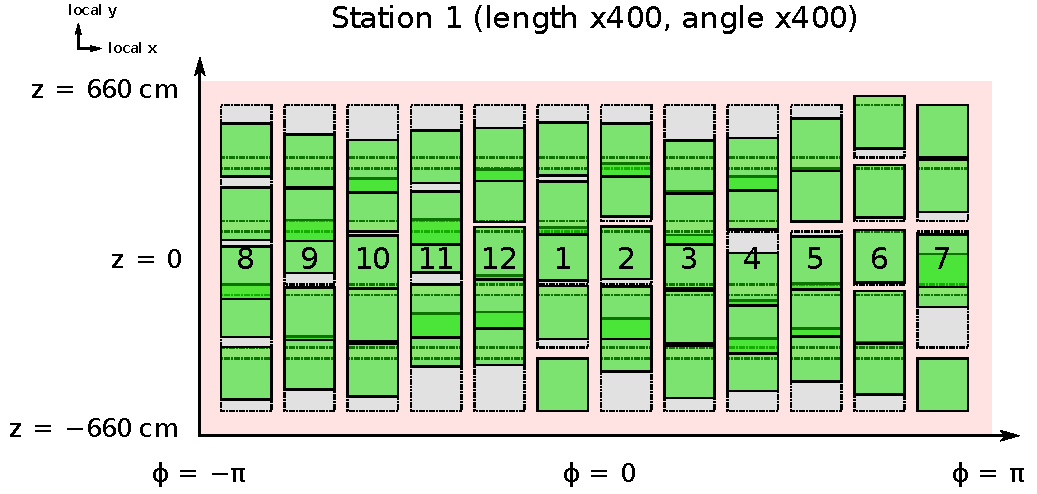
\includegraphics[width=0.5\linewidth]{localy_station1.pdf}

\caption{Exaggerated differences between ``twist'' (left) and
  ``$z$-differences'' (right) geometries and ideal, shown for station~1 in
  an unrolled-barrel view (compare with
  Fig.~\ref{fig:twist3}). \label{fig:twist_station1}}
\end{figure}

{\bf Improvement 1: re-reconstruct tracks from scratch with the new
  geometry, rather than using the track refitter.}

{\bf Improvement 2: use standard $Z'$ samples and resolution
  infrastructure, rather than the privately generated samples and
  ntuples that I used.}

Figure~\ref{fig:curvbias_vseta_ideal_1100_GlobalMuons2} presents the
first result: the effect of the twist on the GlobalMuon curvature
measurement from a 1.1~TeV/$c^2$ $Z'$.  Since the twist is a linear
trend in $r\phi$ hit offsets versus $z$ in the muon system, it causes
a linear trend in curvature bias ($\kappa_\s{refit} - \kappa_\s{gen}$)
versus $\eta$.  (The proper abscissa to quantify a $z$-trend at a
constant distance from the beamline is $\cot\theta$, but $\cot\theta =
\eta + \mathcal{O}(\eta^3)$).  The linear trend from the systematic
misalignment has a comparable width to the intrinsic resolution seen
in the ideal alignment.  At $\eta=\pm 1$, there is an additional
smearing due to tracks that cross the gap between the barrel and the
endcap, since the endcap was not misaligned.  This is an artificial
situation: the endcap will be aligned in a way that matches the
barrel, and therefore this smearing is overly pessimistic.

{\bf Improvement 2: study the effect with the endcap twisted by the
  same amount as the barrel.}

\begin{figure}
\includegraphics[height=0.5\linewidth, angle=90]{curvbias_vseta_ideal_1100_GlobalMuons2.pdf}
\includegraphics[height=0.5\linewidth, angle=90]{curvbias_vseta_twist0_5mrad_1100_GlobalMuons2.pdf}

\caption{Curvature errors vs.\ $\eta$ for a perfectly aligned system
  (left) and a muon system with a twisted barrel (right).  The effect
  of the twist (linear trend) is comparable to the intrinsic momentum
  resolution (vertical spread).  The artificial spread at $\eta = \pm
  1$ is due to tracks that cross the gap between the coherently
  misaligned barrel and the perfectly aligned
  endcap. \label{fig:curvbias_vseta_ideal_1100_GlobalMuons2}}
\end{figure}

The effect of the twist behaves as expected when applied to
higher-momentum muons or reversed
(Fig.~\ref{fig:curvbias_vseta_twist0_5mrad_2000_GlobalMuons2}).
Doubling the muon momentum increases the curvature bias only from
0.16~$c$/TeV/$\eta$ to 0.2~$c$/TeV/$\eta$, as it is approaching a
constant bias in the high-momentum limit: see also
Fig.~\ref{fig:curvbias_vspt_ideal_GlobalMuons2}.  Reversing the twist
of the underlying geometry reverses the slope of the curvature bias,
demonstrating that it is a tunable parameter.

\begin{figure}
\includegraphics[height=0.5\linewidth, angle=90]{curvbias_vseta_twist0_5mrad_2000_GlobalMuons2.pdf}
\includegraphics[height=0.5\linewidth, angle=90]{curvbias_vseta_antitwist0_5mrad_2000_GlobalMuons2.pdf}

\caption{Curvature errors vs.\ $\eta$ for muons from a 2~TeV/$c^2$
  $Z'$ in the twist geometry (left) and the anti-twist geometry
  (right). \label{fig:curvbias_vseta_twist0_5mrad_2000_GlobalMuons2}}
\end{figure}

\begin{figure}
\includegraphics[height=0.5\linewidth, angle=90]{curvbias_vspt_ideal_GlobalMuons2.pdf}
\includegraphics[height=0.5\linewidth, angle=90]{curvbias_vspt_twist0_5mrad_GlobalMuons2.pdf}

\caption{Curvature bias vs.\ $p_T$ for muons from all three $Z'$
  samples (superimposed) in a slice of high $\eta$.  Left: ideal
  geometry; right: twisted geometry.  The effect is {\it not}
  proportional to $p_T$. \label{fig:curvbias_vspt_ideal_GlobalMuons2}}
\end{figure}

To quantify the effect on both $p_T$ and $\eta$, curvature bias was
plotted as a 2-D profile in
Fig.~\ref{fig:trackdistort2d_twist0_5mrad_GlobalMuons2}.  The
dependence on $p_T$ is approximately linear but not proportional,
while the dependence on $\eta$ is proportional.  This is because it is
a (very smooth, broad) threshold effect in $p_T$: when the sagitta of
tracks is larger than the tracker measurements' resolution, the
effective weight of the muon hits in the track-fit is negligible, and
when the sagitta is much smaller than the tracker can measure by
itself, the curvature bias is proportional to the hit-position bias
and not the momentum of the track.  This threshold is set by the
radius and hit resolution of the tracker.

\begin{figure}
\includegraphics[height=\linewidth, angle=90]{trackdistort2d_twist0_5mrad_GlobalMuons2.pdf}
\caption{Curvature bias (color scale) vs.\ $p_T$ and $\eta$ with a 2-D
  fit represented by contour lines.  The color of each pixel
  represents the mean curvature bias in that
  bin. \label{fig:trackdistort2d_twist0_5mrad_GlobalMuons2}}
\end{figure}

Finally, the effects on three TeV-muon reconstruction algorithms are
compared in
Fig.~\ref{fig:curvbias_vseta_twist0_5mrad_1100_GlobalMuons2}.  The
misalignment effect is largely independent of reconstruction algorithm.

\begin{figure}
\includegraphics[height=0.32\linewidth, angle=90]{curvbias_vseta_twist0_5mrad_1100_GlobalMuons2.pdf}
\includegraphics[height=0.32\linewidth, angle=90]{curvbias_vseta_twist0_5mrad_1100_TeVMuons2picky.pdf}
\includegraphics[height=0.32\linewidth, angle=90]{curvbias_vseta_twist0_5mrad_1100_TeVMuons2firstHit.pdf}

\caption{Curvature vs.\ $\eta$ for GlobalMuons (left), the Picky
  track-fit (middle), and the FirstStation track-fit
  (right). \label{fig:curvbias_vseta_twist0_5mrad_1100_GlobalMuons2}}
\end{figure}

\section{Studies of $\eta$ resolution}

The track-based/hardware alignment discrepancies in the global $z$
direction are also on the order of a few millimeters and significantly
affect $\eta$ reconstruction for TeV-scale muons.  These errors in
$\eta$ negligibly affect $Z'$ mass, as we will see in the next
section.

The ``$z$-differences'' geometry prepared for this study includes both
the systematic effect ($z$-length of the barrel) and the
individual-chamber variations because the latter are evident in a plot
of alignment residuals with sharp discrepancies at the boundaries (no
long-distance propagation effect can account for discontinuities
exactly at the chamber boundaries).  Since the individual-chamber
errors are in the model, we can see them in a plot of $\eta$ bias as a
function of $\eta$ and $\phi$, which maps the barrel in
track-parameter bias (Fig.~\ref{fig:etadistort_GlobalMuons2}).  The
net effect of these misalignments smears the $\eta^\s{measured} -
\eta^\s{true}$ distribution by $1\times 10^{-4}$--$1\times 10^{-3}$
(same Figure).  Performing the same study with FirstStation refits
instead of GlobalMuons (Fig.~\ref{fig:etadistort_TeVMuons2firstHit})
reduces the bias and simplifies the $\eta$-$\phi$ map, since tracks
are no longer being affected by muon chambers in different stations.

\begin{figure}
\includegraphics[height=0.5\linewidth, angle=90]{etadistort_GlobalMuons2.pdf}
\includegraphics[height=0.5\linewidth, angle=90]{eta1d_GlobalMuons2.pdf}

\caption{Left: $\eta^\s{measured} - \eta^\s{true}$ (color scale) in
  GlobalMuons from all three $Z'$ samples vs.\ $\eta$ and $p_T$.
  Right: histogram of $\eta^\s{measured} - \eta^\s{true}$ for the same
  samples, same geometry
  distortion. \label{fig:etadistort_GlobalMuons2}}
\end{figure}

\begin{figure}
\includegraphics[height=0.5\linewidth, angle=90]{etadistort_TeVMuons2firstHit.pdf}
\includegraphics[height=0.5\linewidth, angle=90]{eta1d_TeVMuons2firstHit.pdf}

\caption{Left: $\eta^\s{measured} - \eta^\s{true}$ (color scale) in
  FirstStation from all three $Z'$ samples vs.\ $\eta$ and $p_T$.
  Right: histogram of $\eta^\s{measured} - \eta^\s{true}$ for the same
  samples, same geometry
  distortion. \label{fig:etadistort_TeVMuons2firstHit}}
\end{figure}

\section{Studies of $Z'$ mass resolution}

The bottom line for $Z'$ studies is the mass resolution, which is most
conveniently expressed as a percent: $(m^\s{measured} -
m^\s{true})/m^\s{true}$.  We want to see what effect the twist has on
$Z'$ mass thorugh momentum mismeasurement of its daughters, but the
twist effect is highly dependent on $\eta$ and the two muons may have
very different $\eta$ values.  The most useful abscissa in this case
is the $\eta$ difference of the daughters, since the two muons
encounter correlated effects that cancel in mass bias when they sample
the detector at similar $\eta$ values.  More precisely, the mass bias
is a function of

\[ \Delta\eta = q_\s{lead} \, \bigg( \eta_\s{lead} - \eta_\s{sublead} \bigg) \]

{\bf Improvement 3: this should probably be $\eta_{\mu^+} - \eta_{\mu^-}$.}

\noindent where ``lead'' and ``sublead'' refer to the highest-$p_T$ and
second-highest-$p_T$ muons, respectively.
Figure~\ref{fig:massbias_ideal_1100_GlobalMuons2_plus} shows the trend
in mass bias due to a twist.  Since only the barrel has been twisted,
an $|\eta| < 1$ cut has been applied to each muon.

{\bf Improvement 4: $|\eta| < 1$ might not have been far enough:
  Fig.~\ref{fig:curvbias_vseta_ideal_1100_GlobalMuons2} shows that the
  tracks are already beginning to smear due to the artificial
  barrel-endcap mismatch by $|\eta| = 1$.  Doing the study with
  continuity between the barrel and endcap would solve that problem.}

\begin{figure}
\includegraphics[height=0.49\linewidth, angle=90]{massbias_ideal_1100_GlobalMuons2_plus.pdf}
\includegraphics[height=0.49\linewidth, angle=90]{massbias_twist0_5mrad_1100_GlobalMuons2_plus.pdf}
\caption{Mass bias vs.\ $\eta$ difference of the daughters for events
  with $\mu^+$ having the highest $p_T$ (1.1~TeV/$c^2$ $Z'$); for each
  muon, we require $|\eta| < 1$.  Left: ideal geometry; right: twist
  geometry. \label{fig:massbias_ideal_1100_GlobalMuons2_plus}}
\end{figure}

The shape of the mass bias in
Fig.~\ref{fig:massbias_ideal_1100_GlobalMuons2_plus} is not exactly
linear, but it is approximately linear near $\Delta \eta \to 0$.  The
non-linear edges may be related to clipping the distribution with the
$|\eta|$ cut on each muon, as illustrated in Fig.~\ref{fig:clipping}.

\begin{figure}
\begin{center}
\includegraphics[width=0.5\linewidth]{clipping.pdf}
\end{center}
\caption{By applying an $|\eta| < 1$ cut on each muon, we sample a
  different distribution of the box as $\Delta\eta$ varies. \label{fig:clipping}}
\end{figure}

Figure~\ref{fig:massbias_twist0_5mrad_1100_GlobalMuons2_plus}
presents the effect of replacing the leading $\mu^+$ muon with
$\mu^-$: the direction of the trend is reversed.
Figure~\ref{fig:massbias_twist0_5mrad_1100_GlobalMuons2_plus} shows
the distribution with opposite twists: again, the direction is
reversed.  The twist parameter directly tunes the mass bias as a
function of $\Delta \eta$.

\begin{figure}
\includegraphics[height=0.5\linewidth, angle=90]{massbias_twist0_5mrad_1100_GlobalMuons2_plus.pdf}
\includegraphics[height=0.5\linewidth, angle=90]{massbias_twist0_5mrad_1100_GlobalMuons2_minus.pdf}

\caption{Mass bias vs.\ $\Delta \eta$ (1.1~TeV/$c^2$ $Z'$) for $\mu^+$
  having the highest $p_T$ (left) and $\mu^-$ having the highest $p_T$
  (right). \label{fig:massbias_twist0_5mrad_1100_GlobalMuons2_plus}}
\end{figure}

\begin{figure}
\includegraphics[height=0.5\linewidth, angle=90]{massbias_twist0_5mrad_1100_GlobalMuons2_plus.pdf}
\includegraphics[height=0.5\linewidth, angle=90]{massbias_antitwist0_5mrad_1100_GlobalMuons2_plus.pdf}

\caption{Same as
  Figs.~\ref{fig:massbias_ideal_1100_GlobalMuons2_plus} and
  \ref{fig:massbias_twist0_5mrad_1100_GlobalMuons2_plus} for
  opposite-direction twists. \label{massbias_antitwist0_5mrad_1100_GlobalMuons2_plus}}
\end{figure}

Since $Z'$ has a known $\eta$ distribution, we can summarize the
effect of the mass bias on the overall resolution of a $Z'$ peak.
This is shown in Fig.~\ref{fig:massdistribution_1100_GlobalMuons2} for
the 1.1, 2, and 3~TeV/$c^2$ $Z'$ samples.  The $z$-differences
geometry has negligible effect on the $Z'$ mass resolution because the
uncertainty is dominated by muon momentum magnitudes, not directions.
The twist has a significant effect on the mass resolution that grows
with mass.

{\bf Improvement 5: this is where the ``40\%'' figure comes from: the
  1.1~TeV/$c^2$ $Z'$ peak is deflated about 40\% with respect to ideal
  geometry.  How this compares with randomly but not systematically
  misaligned geometry has not yet been tested, but that would be more
  relevant than the 40\% figure, since we really should be quantifying
  the difference between the best it might actually be and the worst
  it might actually be.  We know that the geometry is not ideal.}

{\bf Improvement 6: moreover, the $|\eta| < 1$ cut I apply not only
  gives an incomplete picture of the resolution, but it might not be
  tight enough to avoid the artificial effect of DT-CSC mismatch.  The
  3~TeV/$c^2$ $Z'$ has a significantly different $\eta$ distribution:
  it was less central than the 1.1 and 2~TeV$/c^2$ samples, which
  means that more of it samples the artificial smearing at $|\eta|
  \approx 1$.  Actually, that sounds wrong, too: shouldn't higher-mass
  $Z'$ bosons decay more centrally?}

\begin{figure}
\includegraphics[height=0.32\linewidth, angle=90]{massdistribution_1100_GlobalMuons2.pdf}
\includegraphics[height=0.32\linewidth, angle=90]{massdistribution_2000_GlobalMuons2.pdf}
\includegraphics[height=0.32\linewidth, angle=90]{massdistribution_3000_GlobalMuons2.pdf}

\caption{Mass resolution of $Z'$ with ideal geometry (black),
  $z$-differences geometry (dashed red), and twist (dotted blue).
  Left is 1.1~TeV/$c^2$, middle is 2~TeV/$c^2$, and right is
  3~TeV/$c^2$ and all three require $|\eta| < 1$ for both daughters.
  The $z$-differences geometry, affecting only the $\eta$ of global
  tracks, has negligible effect on the $Z'$ mass resolution.  The
  effect of the twist geometry is significant and grows with $Z'$
  mass. \label{fig:massdistribution_1100_GlobalMuons2}}
\end{figure}

\section{Conclusions}

The main improvement is to include more than one effect: not just the
barrel twist, but also how the endcap would follow the ends of the
barrel.  Many of the items labeled ``improvement'' above are different
aspects of that one deficiency.  Also, we will have systematic
misalignment models of the endcap as well, and they should be included
on an equal footing in the study.  The ``$z$-differences'' test does
not need to be repeated: it is irrelevant.

Ultimately, the only thing that is really needed is the 1-D mass
resolution plot.  However, I think that ``monitoring'' the effect as a
function of kinematic variables shows that we have an understanding of
the detector issues that cause it and we can be more confident that
``$x$ amount of misalignment uncertainty about some parameter yields
$y$ mass resolution smearing.''  I've already found most of the
relevant variables: they can be added to an ntuple rather easily.

\end{document}
